\section{Desenvolvimento}

Sed lacinia nulla vitae enim. Pellentesque tincidunt purus vel magna.
Integer non enim. Praesent euismod nunc eu purus. Donec bibendum quam in tellus.
Nullam cursus pulvinar lectus. Donec et mi. Nam vulputate metus eu enim. Vestibulum
pellentesque felis eu massa. \\

\begin{figure}[h]
    \centering
    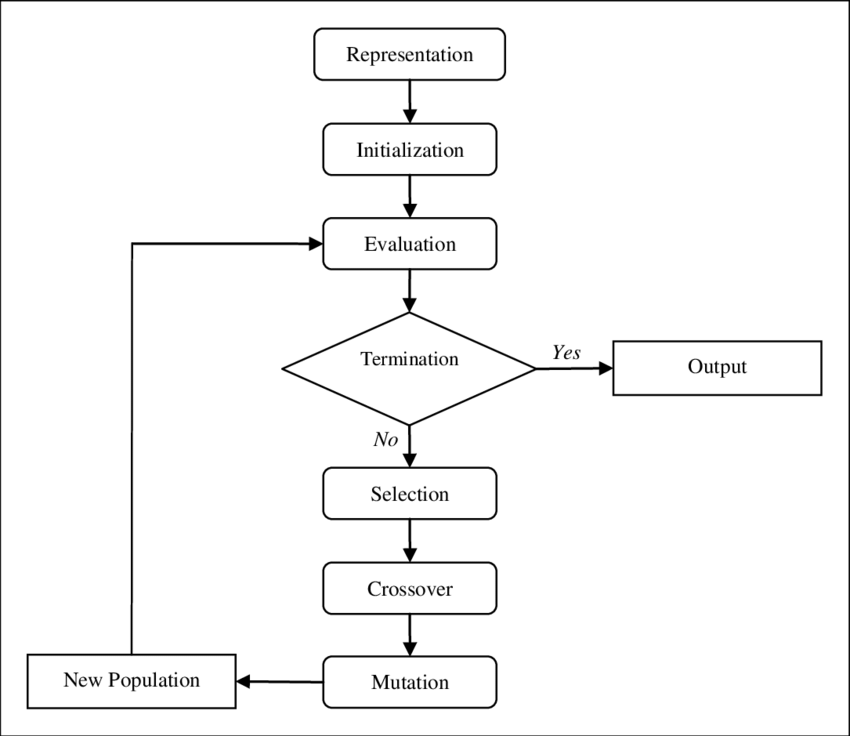
\includegraphics[width=0.75\textwidth]{images/Steps-of-Genetic-Algorithms.png}
    \caption{Laamarti, Eid e El Saddik, Acredite}
\end{figure}

\subsection{Item do Desenvolvimento}

Nam dui ligula, fringilla a, euismod sodales, sollicitudin vel, wisi. Morbi auctor lorem non
justo. Nam lacus libero, pretium at, lobortis vitae, ultricies et, tellus. Donec aliquet, tortor
sed accumsan bibendum, erat ligula aliquet magna, vitae ornare odio metus a mi. Morbi
ac orci et nisl hendrerit mollis. Suspendisse ut massa. Cras nec ante. Pellentesque a nulla.
Cum sociis natoque penatibus et magnis dis parturient montes, nascetur ridiculus mus.
Aliquam tincidunt urna. Nulla ullamcorper vestibulum turpis. Pellentesque cursus luctus
mauris. \\

Nulla malesuada porttitor diam. Donec felis erat, congue non, volutpat at, tincidunt
tristique, libero. Vivamus viverra fermentum felis. Donec nonummy pellentesque ante.
Phasellus adipiscing semper elit. Proin fermentum massa ac quam. Sed diam turpis,
molestie vitae, placerat a, molestie nec, leo. Maecenas lacinia. Nam ipsum ligula, eleifend
at, accumsan nec, suscipit a, ipsum. Morbi blandit ligula feugiat magna. Nunc eleifend
consequat lorem. Sed lacinia nulla vitae enim. Pellentesque tincidunt purus vel magna.
Integer non enim. Praesent euismod nunc eu purus. Donec bibendum quam in tellus.
Nullam cursus pulvinar lectus. Donec et mi. Nam vulputate metus eu enim. Vestibulum
pellentesque felis eu massa. \\

Fusce mauris. Vestibulum luctus nibh at lectus. Sed bibendum, nulla a faucibus semper, leo
velit ultricies tellus, ac venenatis arcu wisi vel nisl. Vestibulum diam. Aliquam pellentesque,
augue quis sagittis posuere, turpis lacus congue quam, in hendrerit risus eros eget felis.
Maecenas eget erat in sapien mattis porttitor. Vestibulum porttitor. Nulla facilisi. Sed a
turpis eu lacus commodo facilisis. Morbi fringilla, wisi in dignissim interdum, justo lectus
sagittis dui, et vehicula libero dui cursus dui. Mauris tempor ligula sed lacus. Duis cursus
enim ut augue. Cras ac magna. Cras nulla. Nulla egestas. Curabitur a leo. Quisque egestas
wisi eget nunc. Nam feugiat lacus vel est. Curabitur consectetuer. \\

\subsection{Item do Desenvolvimento}

Fusce mauris. Vestibulum luctus nibh at lectus. Sed bibendum, nulla a faucibus semper, leo
velit ultricies tellus, ac venenatis arcu wisi vel nisl. Vestibulum diam. Aliquam pellentesque,
augue quis sagittis posuere, turpis lacus congue quam, in hendrerit risus eros eget felis.
Maecenas eget erat in sapien mattis porttitor. Vestibulum porttitor. Nulla facilisi. Sed a
turpis eu lacus commodo facilisis. Morbi fringilla, wisi in dignissim interdum, justo lectus
sagittis dui, et vehicula libero dui cursus dui. Mauris tempor ligula sed lacus. Duis cursus
enim ut augue. Cras ac magna. Cras nulla. Nulla egestas \cite{einstein}. Curabitur a leo. Quisque egestas
wisi eget nunc. Nam feugiat lacus vel est. Curabitur consectetuer. \\

$$
f(t) = \frac{1}{2\pi} \int_{-\infty}^{\infty} F(\omega) \, e^{i\omega t} \, d\omega
$$ \\

Sed lacinia nulla vitae enim. Pellentesque tincidunt purus vel magna.
Integer non enim. Praesent euismod nunc eu purus. Donec bibendum quam in tellus.
Nullam cursus pulvinar lectus. Donec et mi. Nam vulputate metus eu enim. Vestibulum
pellentesque felis eu massa. \\

Fusce mauris. Vestibulum luctus nibh at lectus. Sed bibendum, nulla a faucibus semper, leo
velit ultricies tellus, ac venenatis arcu wisi vel nisl. Vestibulum diam. Aliquam pellentesque,
augue quis sagittis posuere, turpis lacus congue quam, in hendrerit risus eros eget felis.
Maecenas eget erat in sapien mattis porttitor. Vestibulum porttitor. Nulla facilisi. Sed a
turpis eu lacus commodo facilisis. Morbi fringilla, wisi in dignissim interdum, justo lectus
sagittis dui, et vehicula libero dui cursus dui. Mauris tempor ligula sed lacus. Duis cursus
enim ut augue. Cras ac magna. Cras nulla. Nulla egestas. Curabitur a leo. Quisque egestas
wisi eget nunc. Nam feugiat lacus vel est. Curabitur consectetuer. \\

\begin{figure}[h]
    \centering
    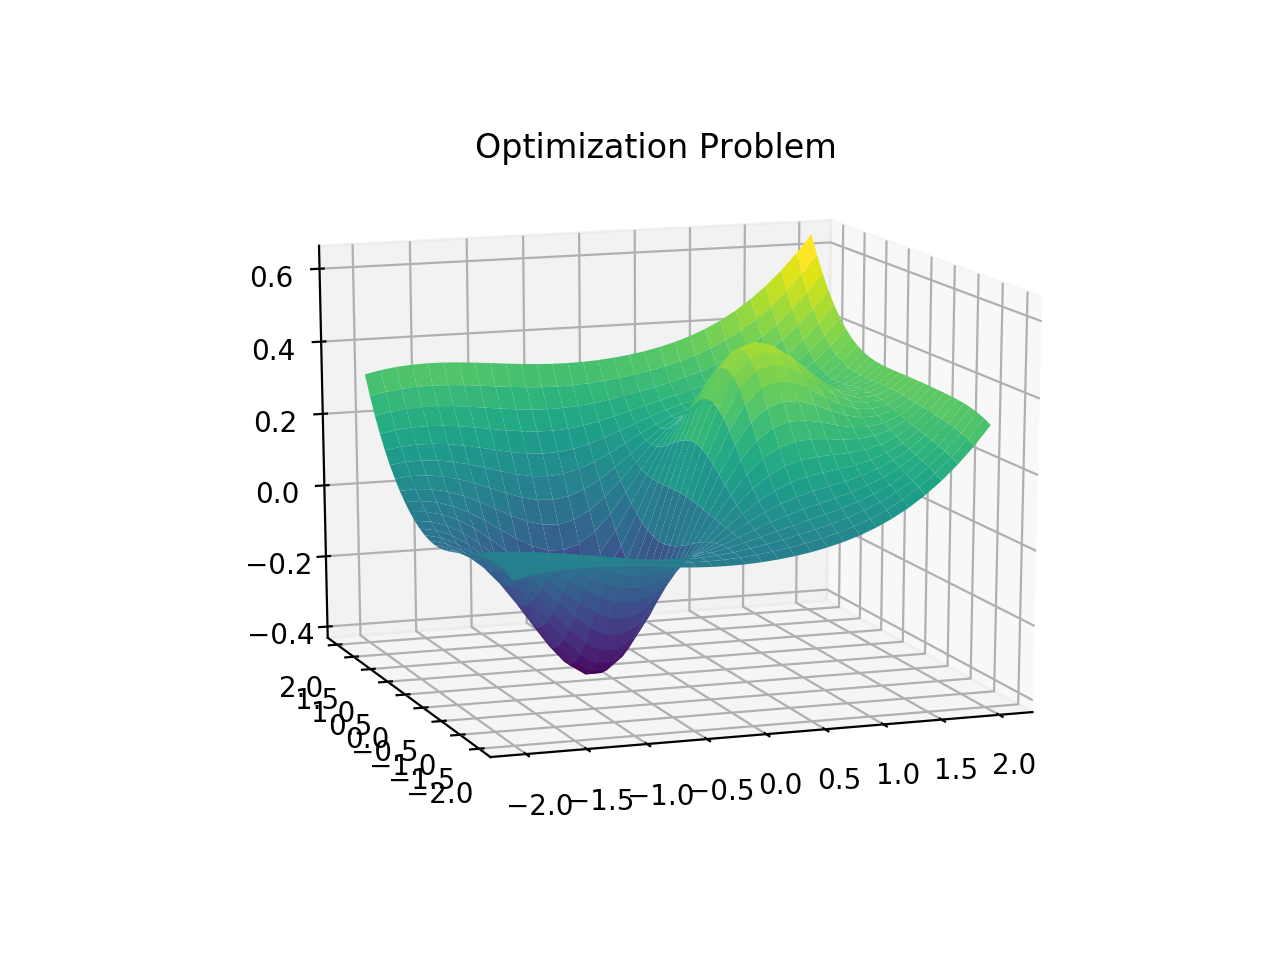
\includegraphics[width=0.75\textwidth]{images/plot2.png}
    \caption{Laamarti, Eid e El Saddik, Acredite}
\end{figure}

Sed lacinia nulla vitae enim. Pellentesque tincidunt purus vel magna.
Integer non enim. Praesent euismod nunc eu purus. Donec bibendum quam in tellus.
Nullam cursus pulvinar lectus. Donec et mi. Nam vulputate metus eu enim. Vestibulum
pellentesque felis eu massa. \\

\subsubsection{Subitem do Desenvolvimento}

Fusce mauris. Vestibulum luctus nibh at lectus. Sed bibendum, nulla a faucibus semper, leo
velit ultricies tellus, ac venenatis arcu wisi vel nisl. Vestibulum diam. Aliquam pellentesque,
augue quis sagittis posuere, turpis lacus congue quam, in hendrerit risus eros eget felis.
Maecenas eget erat in sapien mattis porttitor. Vestibulum porttitor. Nulla facilisi. Sed a
turpis eu lacus commodo facilisis. Morbi fringilla, wisi in dignissim interdum, justo lectus
sagittis dui, et vehicula libero dui cursus dui. Mauris tempor ligula sed lacus. Duis cursus
enim ut augue. Cras ac magna. Cras nulla. Nulla egestas. Curabitur a leo. Quisque egestas
wisi eget nunc. Nam feugiat lacus vel est. Curabitur consectetuer. \\

\begin{figure}[h]
    \centering
    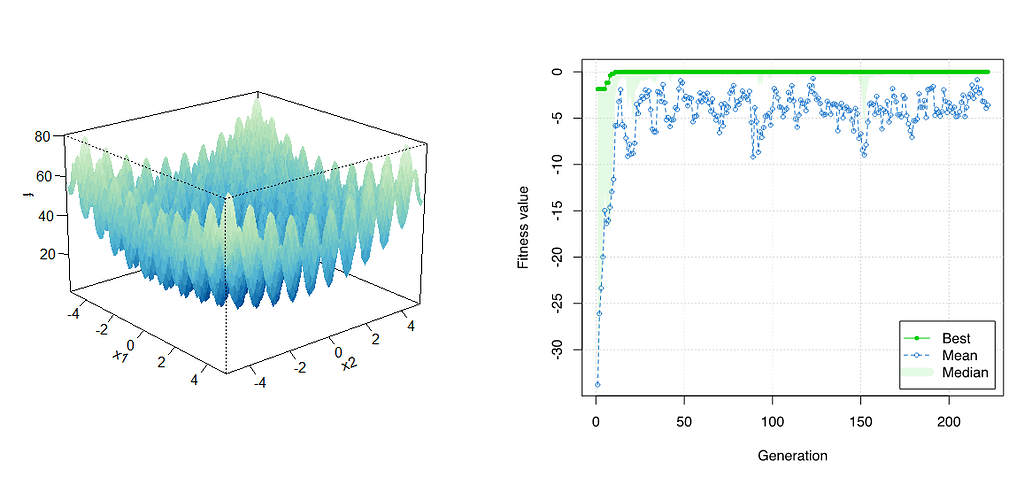
\includegraphics[width=0.65\textwidth]{images/plot.png}
    \caption{Laamarti, Eid e El Saddik, Acredite}
\end{figure}

Sed lacinia nulla vitae enim. Pellentesque tincidunt purus vel magna.
Integer non enim. Praesent euismod nunc eu purus. Donec bibendum quam in tellus.
Nullam cursus pulvinar lectus. Donec et mi. Nam vulputate metus eu enim. Vestibulum
pellentesque felis eu massa. \\



\begin{table}[htbp]
    \centering
    \caption{Exemplo de Conjunto de Dados Aleatórios}
    \begin{tabular}{c c c c c}
    \toprule
    \textbf{ID} & \textbf{Valor 1} & \textbf{Valor 2} & \textbf{Valor 3} & \textbf{Valor 4} \\
    \midrule
    1 & 10 & 5 & 8 & 12 \\
    2 & 25 & 13 & 20 & 28 \\
    3 & 18 & 7 & 10 & 15 \\
    4 & 32 & 16 & 25 & 36 \\
    5 & 15 & 8 & 12 & 18 \\
    \bottomrule
    \end{tabular}
\end{table}

Sed lacinia nulla vitae enim. Pellentesque tincidunt purus vel magna.
Integer non enim. Praesent euismod nunc eu purus.

\subsubsection{Subitem do Desenvolvimento}

Sed lacinia nulla vitae enim. Pellentesque tincidunt purus vel magna.
Integer non enim. Praesent euismod nunc eu purus. Donec bibendum quam in tellus.
Nullam cursus pulvinar lectus. Donec et mi. Nam vulputate metus eu enim. Vestibulum
pellentesque felis eu massa. \\

\begin{itemize}
    \item \textbf{Algoritmo NP-Completo:}
        \begin{itemize}
            \item NP-completo refere-se a uma classe de problemas na teoria da complexidade computacional. 
            \item São difíceis de resolver em termos de tempo computacional, mas fáceis de verificar uma solução caso ela seja proposta.
            \item Exemplo clássico: Problema do Caixeiro Viajante.
        \end{itemize}

    \item \textbf{Problema da Mochila (Knapsack Problem):}
        \begin{itemize}
            \item É um problema de otimização onde o objetivo é escolher um conjunto de itens, cada um com um peso e um valor associado, de forma a maximizar o valor total, sem exceder uma capacidade máxima de peso.
            \item Variantes incluem Problema da Mochila 0-1 (itens não podem ser divididos) e Problema da Mochila Fracionária (itens podem ser divididos).
        \end{itemize}

    \item \textbf{Solução com Algoritmos Genéticos:}
        \begin{itemize}
            \item Algoritmos genéticos são técnicas de otimização baseadas em ideias inspiradas pela evolução biológica. 
            \item São usados para encontrar soluções aproximadas para problemas de otimização complexos. Conforme descrito por \cite{cormen}
            \item Para o Problema da Mochila, os algoritmos genéticos podem ser aplicados da seguinte forma:
            \begin{itemize}
                \item \textbf{Representação}: Cada indivíduo na população é representado como um vetor binário, onde cada bit representa a presença ou ausência de um item na mochila.
                \item \textbf{Função de Aptidão (Fitness)}: A aptidão de um indivíduo é calculada como o valor total dos itens incluídos na mochila, desde que o peso total não exceda a capacidade máxima.
                \item \textbf{Operadores Genéticos}: São aplicados os operadores de seleção, crossover (cruzamento) e mutação para evoluir a população em direção a soluções melhores.
                \item \textbf{Critério de Parada}: A evolução continua até que um critério de parada seja atingido, como um número máximo de gerações ou um valor de aptidão desejado.
            \end{itemize}
        \end{itemize}
\end{itemize}

\subsection{Item do Desenvolvimento}

Sed lacinia nulla vitae enim. Pellentesque tincidunt purus vel magna.
Integer non enim. Praesent euismod nunc eu purus. Donec bibendum quam in tellus.
Nullam cursus pulvinar lectus. Donec et mi. Nam vulputate metus eu enim. Vestibulum
pellentesque felis eu massa. \\

\begin{table}[htbp]
    \centering
    \caption{Exemplo de Conjunto de Dados Aleatórios}
    \begin{tabular}{c c c c c}
    \toprule
    \textbf{ID} & \textbf{Valor 1} & \textbf{Valor 2} & \textbf{Valor 3} & \textbf{Valor 4} \\
    \midrule
    1 & Algoritmo & 10 & 5 & Inteiro \\
    2 & Estrutura de Dados & 25 & 13 & Ponto Flutuante \\
    3 & Programação & 18 & 7 & String \\
    4 & Redes & 32 & 16 & Booleano \\
    5 & Segurança & 15 & 8 & Array \\
    \bottomrule
    \end{tabular}
\end{table}